\documentclass[11pt,a4paper]{article}
\usepackage[utf8]{inputenc}
\usepackage[T1]{fontenc}
\usepackage[french]{babel}
\usepackage{geometry,amsmath,booktabs,graphicx,float,hyperref}
\geometry{margin=2.2cm}
\graphicspath{{../figures/}}

\title{TP d'optimisation avec NumPy}
\author{Mohamed Reda Lakouas}
\date{Octobre 2026}

\begin{document}
\maketitle

\section{Introduction}
Le but de ce TP est de programmer plusieurs méthodes d'optimisation avec NumPy.
J'ai travaillé sur trois problèmes : la régression, la classification et le
clustering. J'ai comparé GD, GD avec recherche du pas, SGD, Momentum, AdaGrad,
RMSprop et Adam.

J'ai utilisé les graines 42, 123 et 2024 pour les petits jeux. Pour MNIST et
Fashion-MNIST, j'ai d'abord fait un essai court avec 3000 images train, 1000
validation et 1000 test. Cet essai utilise une graine et deux époques. Il sert
surtout à vérifier que tout le programme fonctionne.

Le code utilisé pour obtenir les résultats est disponible sur GitHub :
\begin{center}
\url{https://github.com/DevOam/optimisation-numerique-numpy}
\end{center}

\section{Principe de l'optimisation}
Le modèle possède des paramètres notés $\theta$. La fonction $J(\theta)$ mesure
l'erreur. Le gradient indique la direction où cette erreur augmente. Pour la
faire diminuer, j'utilise la mise à jour suivante :
\[
\theta_{nouveau}=\theta_{ancien}-\eta\,\nabla J(\theta).
\]
Le nombre $\eta$ est le pas d'apprentissage. S'il est trop petit, le programme
avance lentement. S'il est trop grand, la perte peut devenir instable.

Dans le code, les sept méthodes utilisent la même boucle. Seule la façon de
modifier le gradient change. Adam utilise par exemple une moyenne du gradient
et une moyenne des gradients au carré.

J'ai aussi vérifié les gradients par différences finies avec $h=10^{-5}$.
Les erreurs obtenues sont entre $10^{-8}$ et $10^{-10}$. Cela montre que les
gradients programmés sont corrects.

\section{Exercice 1 : régression}
Pour OLS et Ridge, la perte utilisée est :
\[
J(w)=\frac{\lVert Xw-y\rVert^2}{2n}+\frac{\lambda}{2}w^TPw.
\]
Quand $\lambda=0$, on obtient OLS. Pour Ridge, $\lambda>0$. Le biais n'est pas
pénalisé. J'ai aussi utilisé le noyau RBF pour représenter une relation non
linéaire.

\begin{table}[H]\centering\small
\caption{Comparaison des sept méthodes avec RBF sur Nonlinear.}
\resizebox{\textwidth}{!}{\begin{tabular}{lrrrrrrrr}\toprule
Méthode & RMSE moyenne $\pm$ écart type & MAE & $R^2$ & Temps (s) & Mises à jour & Gradients & Pertes\\\midrule
GD & $0.683\pm0.000$ & 0.597 & 0.311 & 0.015 & 120 & 120 & 240\\
GD recherche & $0.640\pm0.000$ & 0.560 & 0.396 & 0.015 & 120 & 120 & 240\\
SGD & $0.662\pm0.002$ & 0.579 & 0.354 & 0.050 & 840 & 840 & 240\\
Momentum & $0.575\pm0.003$ & 0.501 & 0.511 & 0.049 & 840 & 840 & 240\\
AdaGrad & $0.592\pm0.002$ & 0.517 & 0.483 & 0.036 & 840 & 840 & 240\\
RMSprop & $0.574\pm0.009$ & 0.502 & 0.514 & 0.039 & 840 & 840 & 240\\
Adam & $0.565\pm0.008$ & 0.487 & 0.529 & 0.045 & 840 & 840 & 240\\\bottomrule
\end{tabular}}
\end{table}

Le résultat principal est que RBF fonctionne mieux sur le jeu Nonlinear. C'est
logique car OLS cherche seulement une relation linéaire. Sur Diabetes, Ridge et
OLS donnent des résultats proches et sont meilleurs que le RBF essayé. Le
meilleur résultat Diabetes est obtenu par Ridge avec Adam : RMSE $=53.740$,
MAE $=42.940$ et $R^2=0.467$.

\begin{figure}[H]\centering
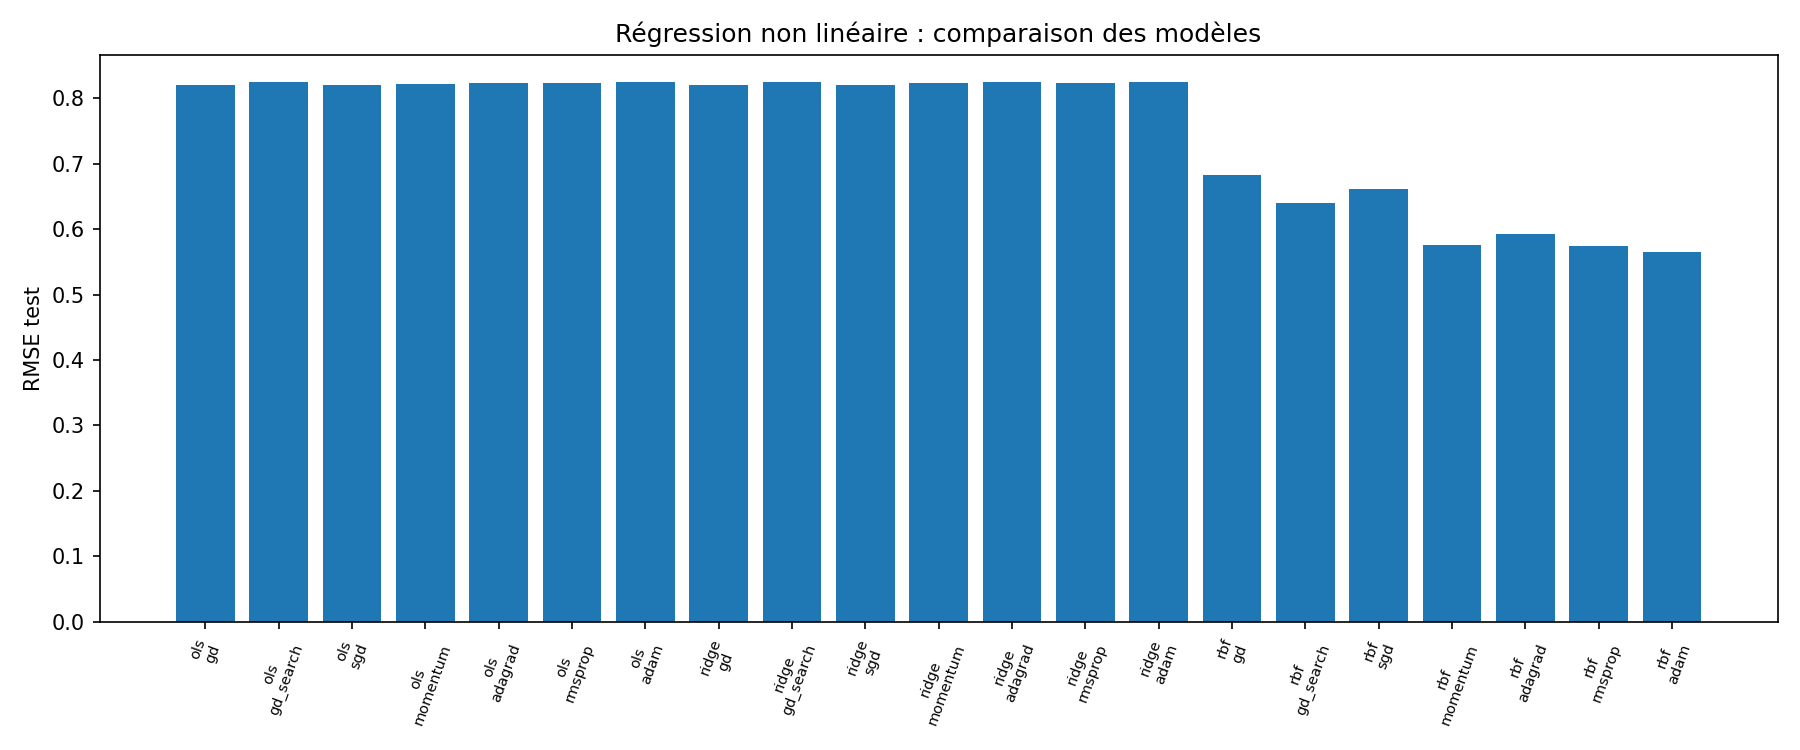
\includegraphics[width=.62\textwidth]{regression_comparaison_rmse.png}
\caption{Comparaison des modèles sur le jeu Nonlinear.}
\end{figure}

\begin{figure}[H]\centering
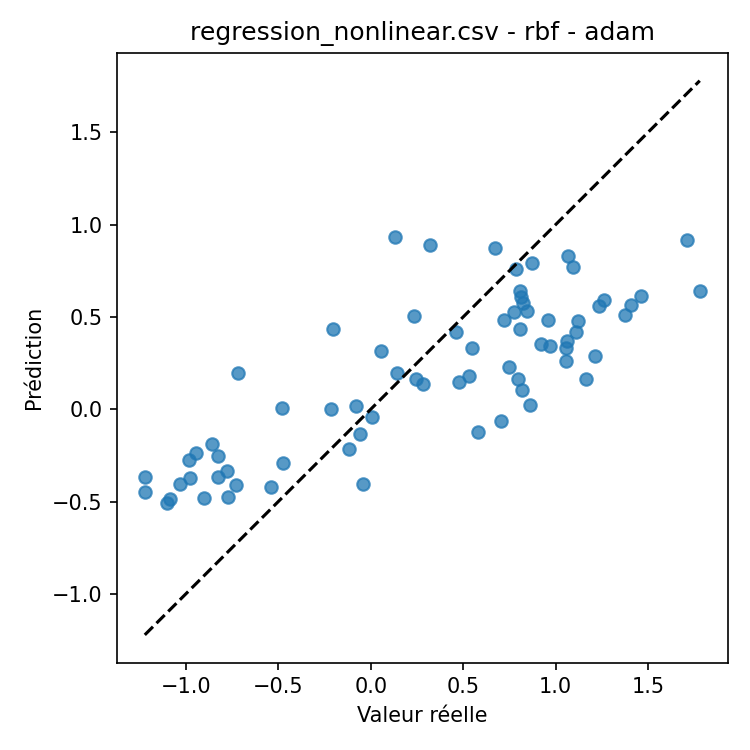
\includegraphics[width=.46\textwidth]{regression_regression_nonlinear_predictions.png}
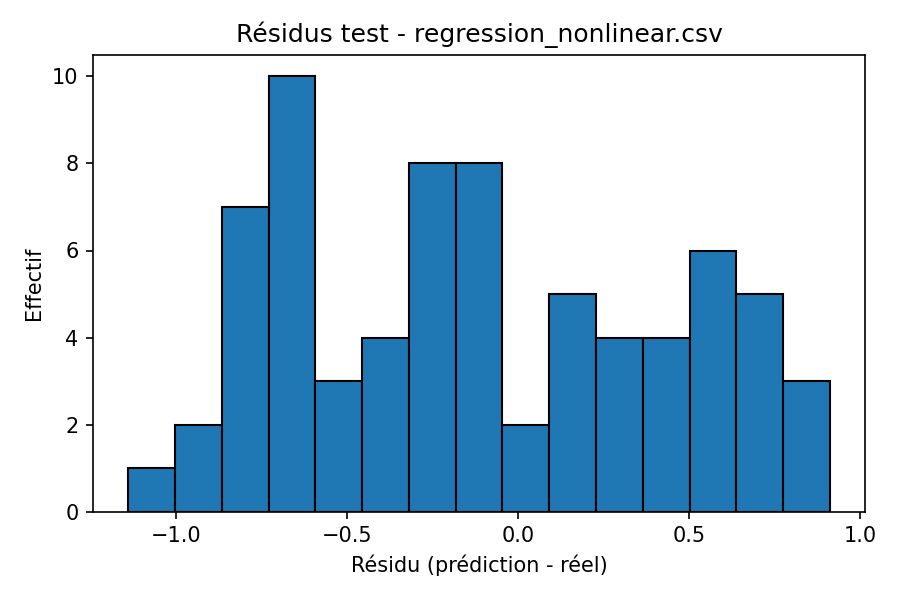
\includegraphics[width=.46\textwidth]{regression_regression_nonlinear_residus.png}
\caption{Prédictions et résidus du meilleur modèle.}
\end{figure}

\section{Exercice 2 : classification}
J'ai programmé un petit réseau avec deux couches cachées. Les architectures sont
$2\to32\to16\to3$ pour Spiral, $4\to32\to16\to3$ pour Iris et
$784\to128\to64\to10$ pour les images. Les couches cachées utilisent $\tanh$.
La dernière couche utilise softmax pour obtenir les probabilités des classes.

\begin{table}[H]\centering\small
\caption{Comparaison des sept méthodes sur Spiral.}
\resizebox{\textwidth}{!}{\begin{tabular}{lrrrrrr}\toprule
Méthode & Exactitude moyenne $\pm$ écart type & Précision macro & Rappel macro & F1 macro & Entropie & Temps (s)\\\midrule
GD & $0.711\pm0.000$ & 0.711 & 0.711 & 0.711 & 0.571 & 0.118\\
GD recherche & $0.989\pm0.000$ & 0.989 & 0.989 & 0.989 & 0.074 & 1.432\\
SGD & $0.726\pm0.005$ & 0.726 & 0.726 & 0.726 & 0.525 & 0.117\\
Momentum & $0.989\pm0.000$ & 0.989 & 0.989 & 0.989 & 0.083 & 0.226\\
AdaGrad & $0.989\pm0.000$ & 0.989 & 0.989 & 0.989 & 0.045 & 0.129\\
RMSprop & $0.989\pm0.000$ & 0.989 & 0.989 & 0.989 & 0.059 & 0.154\\
Adam & $0.989\pm0.000$ & 0.989 & 0.989 & 0.989 & 0.085 & 0.192\\\bottomrule
\end{tabular}}
\end{table}

Sur Spiral, les méthodes adaptatives apprennent mieux la forme des spirales que
GD avec le pas choisi. Pour les images, RMSprop donne le meilleur résultat de
l'essai court. Je ne considère pas ce résultat comme définitif car deux époques
ne suffisent pas pour conclure. Sur Iris, AdaGrad donne 0.944 d'exactitude et de
F1 macro. Dans l'essai images, RMSprop obtient 0.849 sur MNIST et 0.707 sur
Fashion-MNIST.

\begin{figure}[H]\centering
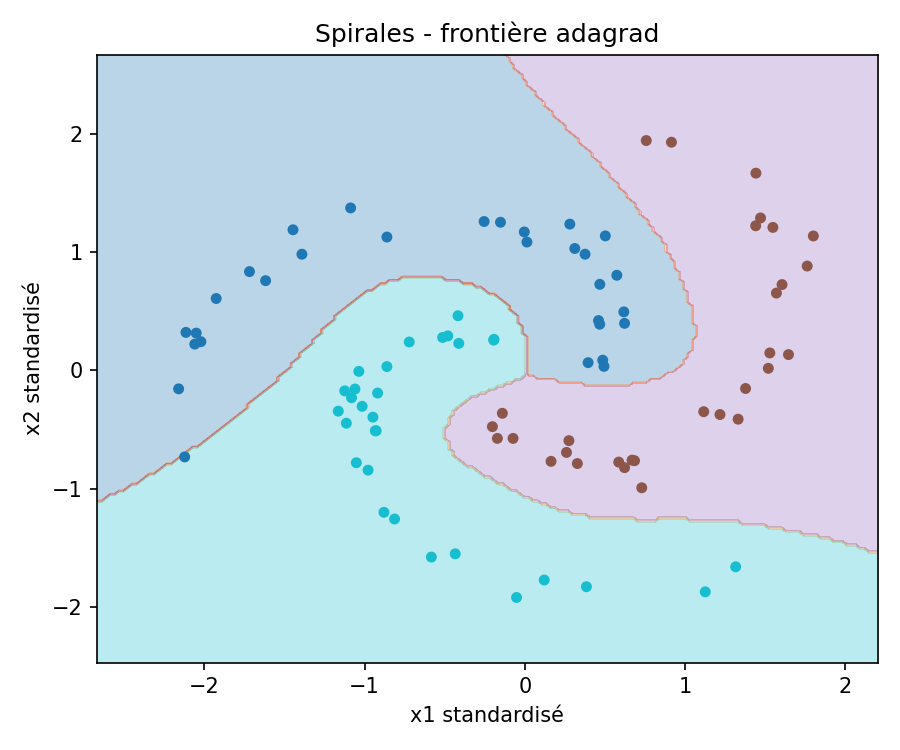
\includegraphics[width=.46\textwidth]{classification_spiral_frontiere.png}
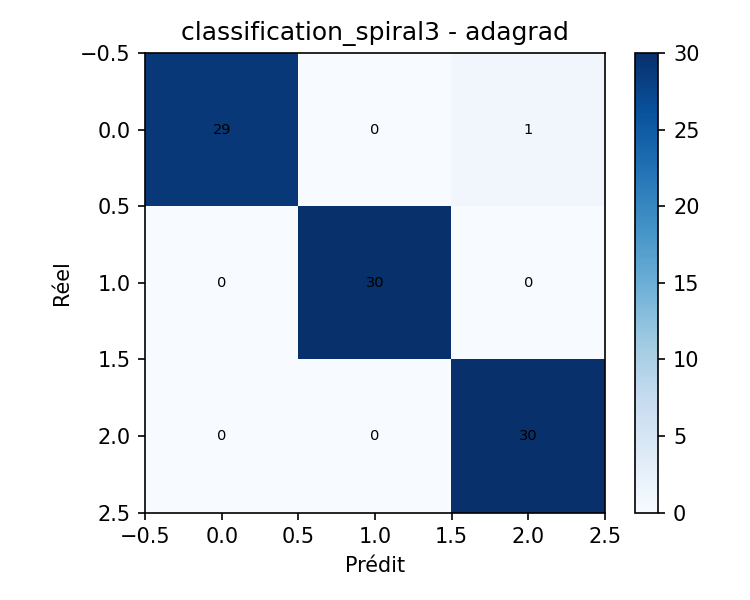
\includegraphics[width=.46\textwidth]{classification_classification_spiral3_confusion.png}
\caption{Frontière de décision et matrice de confusion de Spiral.}
\end{figure}

\begin{figure}[H]\centering
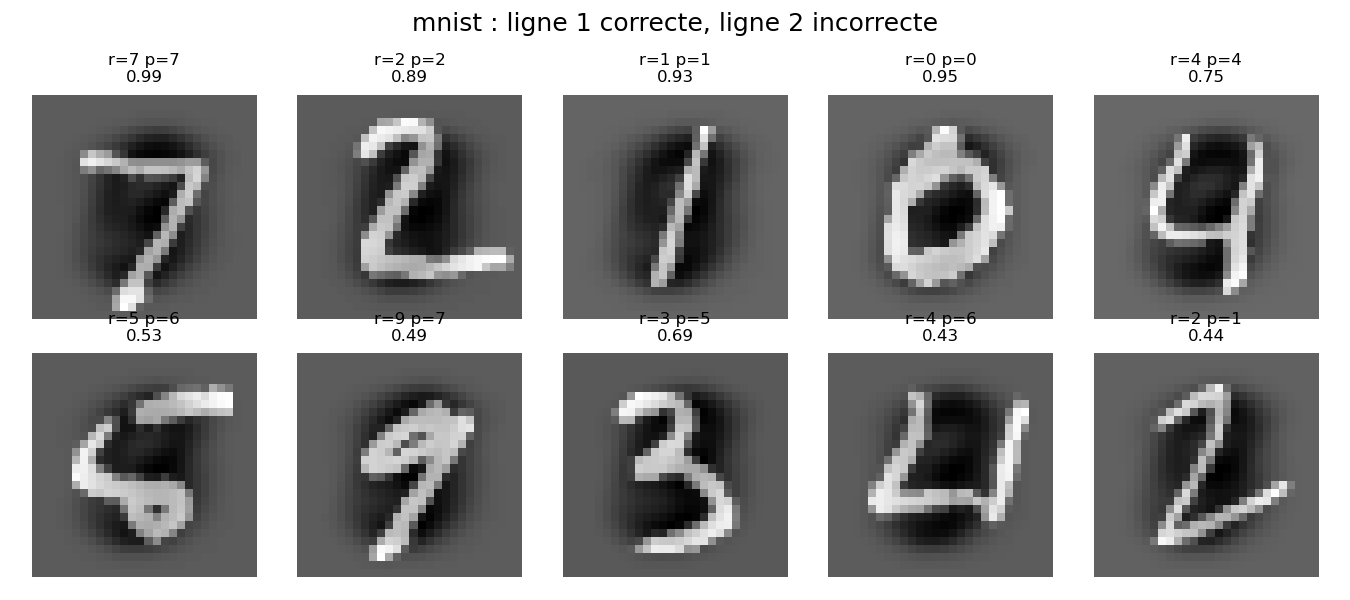
\includegraphics[width=.75\textwidth]{classification_mnist_exemples.png}
\caption{Exemples MNIST bien et mal classés.}
\end{figure}

\section{Exercice 3 : clustering}
Pour éviter un grand tableau en mémoire, les distances sont calculées avec :
\[
D_{ik}=\lVert x_i\rVert^2+\lVert c_k\rVert^2-2x_i^Tc_k.
\]
Les points sont associés de façon douce aux centroïdes pendant l'apprentissage.
À la fin, chaque point reçoit le centroïde le plus proche. Les vraies classes ne
sont utilisées qu'après l'apprentissage pour calculer ARI et NMI. J'ai aussi
programmé Lloyd comme méthode de comparaison.

\begin{table}[H]\centering\small
\caption{Comparaison sur Blobs. Lloyd est ajouté comme référence.}
\resizebox{\textwidth}{!}{\begin{tabular}{lrrrrrr}\toprule
Méthode & Perte & Inertie & Silhouette & ARI $\pm$ écart type & NMI & Temps (s)\\\midrule
GD & 0.656 & 0.383 & 0.676 & $0.970\pm0.014$ & 0.954 & 0.011\\
GD recherche & 0.564 & 0.290 & 0.679 & $0.975\pm0.000$ & 0.960 & 0.095\\
SGD & 0.565 & 0.291 & 0.679 & $0.975\pm0.000$ & 0.960 & 0.023\\
Momentum & 0.564 & 0.290 & 0.679 & $0.975\pm0.000$ & 0.960 & 0.023\\
AdaGrad & 0.565 & 0.291 & 0.679 & $0.975\pm0.000$ & 0.960 & 0.024\\
RMSprop & 0.564 & 0.290 & 0.679 & $0.975\pm0.000$ & 0.960 & 0.024\\
Adam & 0.564 & 0.290 & 0.679 & $0.975\pm0.000$ & 0.960 & 0.025\\
Lloyd & 0.564 & 0.290 & 0.679 & $0.975\pm0.000$ & 0.960 & 0.000\\\bottomrule
\end{tabular}}
\end{table}

Blobs est le jeu le plus facile car ses trois groupes sont bien séparés. Wine
est plus sensible à l'initialisation. Sur les images, Lloyd est meilleur dans
ce petit essai. Une petite inertie ne garantit pas forcément une bonne valeur
d'ARI, car les deux mesures ne représentent pas exactement la même chose.
Sur Wine, le meilleur ARI moyen est 0.897 avec Momentum. Dans les essais images,
Lloyd obtient un ARI de 0.389 sur MNIST et 0.326 sur Fashion-MNIST.

\begin{figure}[H]\centering
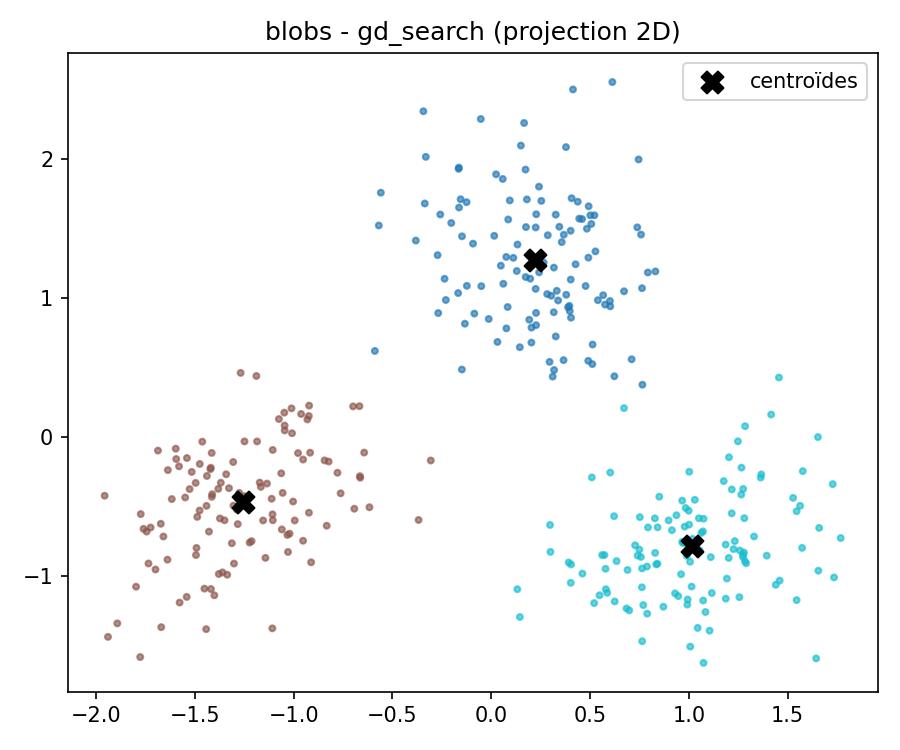
\includegraphics[width=.46\textwidth]{clustering_blobs_projection.png}
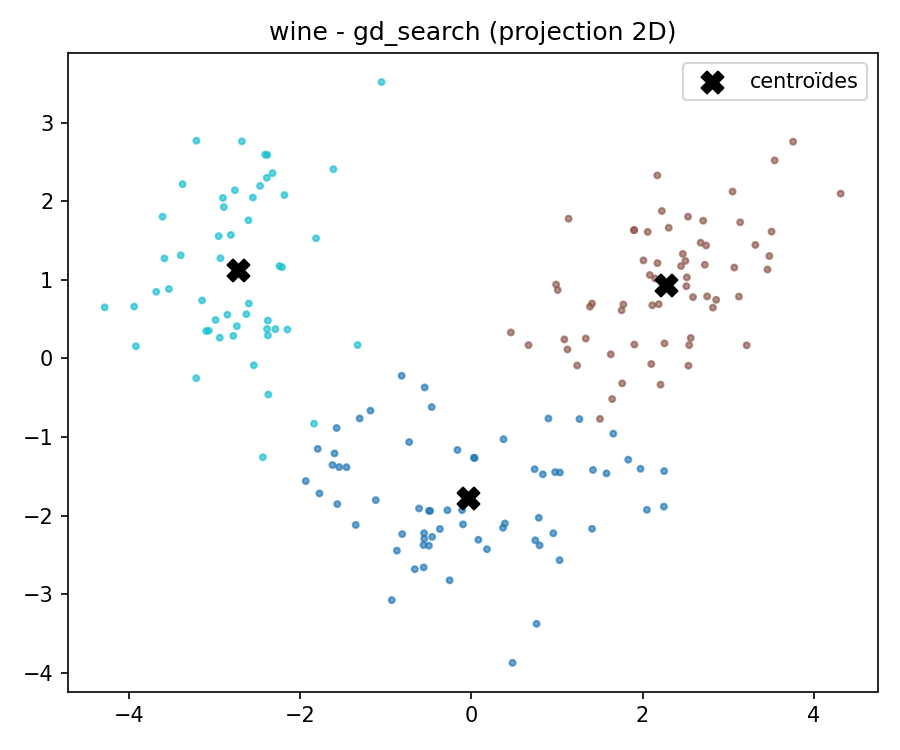
\includegraphics[width=.46\textwidth]{clustering_wine_projection.png}
\caption{Clustering de Blobs et projection PCA de Wine.}
\end{figure}

\begin{figure}[H]\centering
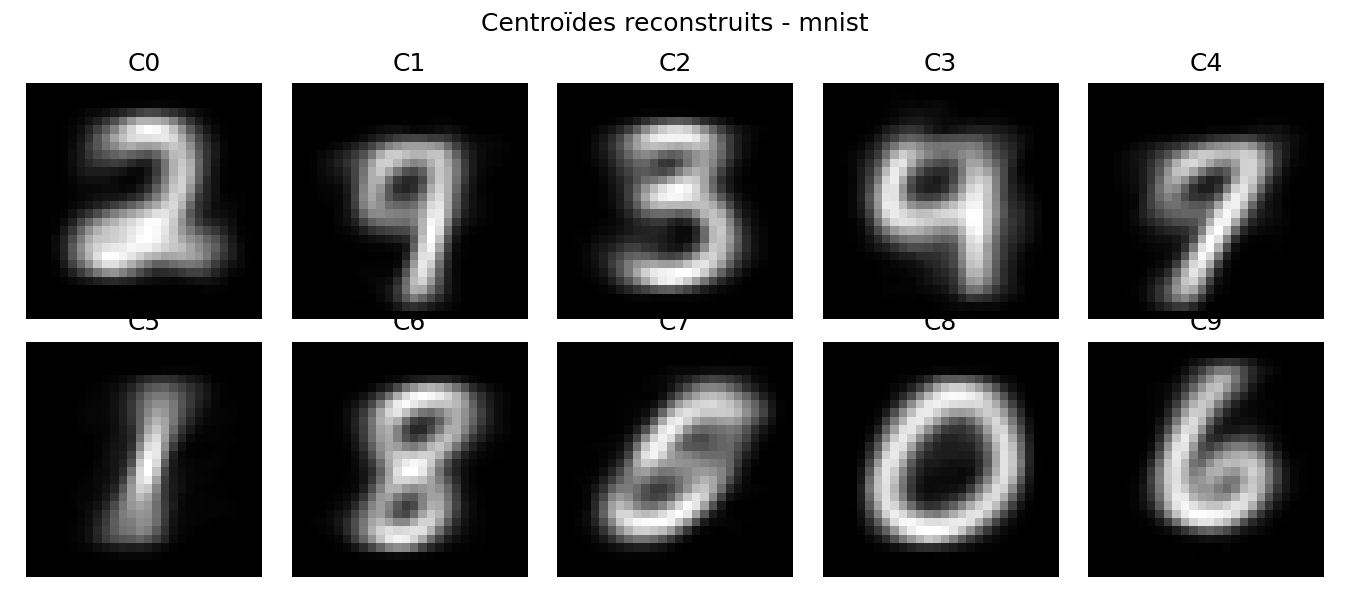
\includegraphics[width=.46\textwidth]{clustering_mnist_centroides.png}
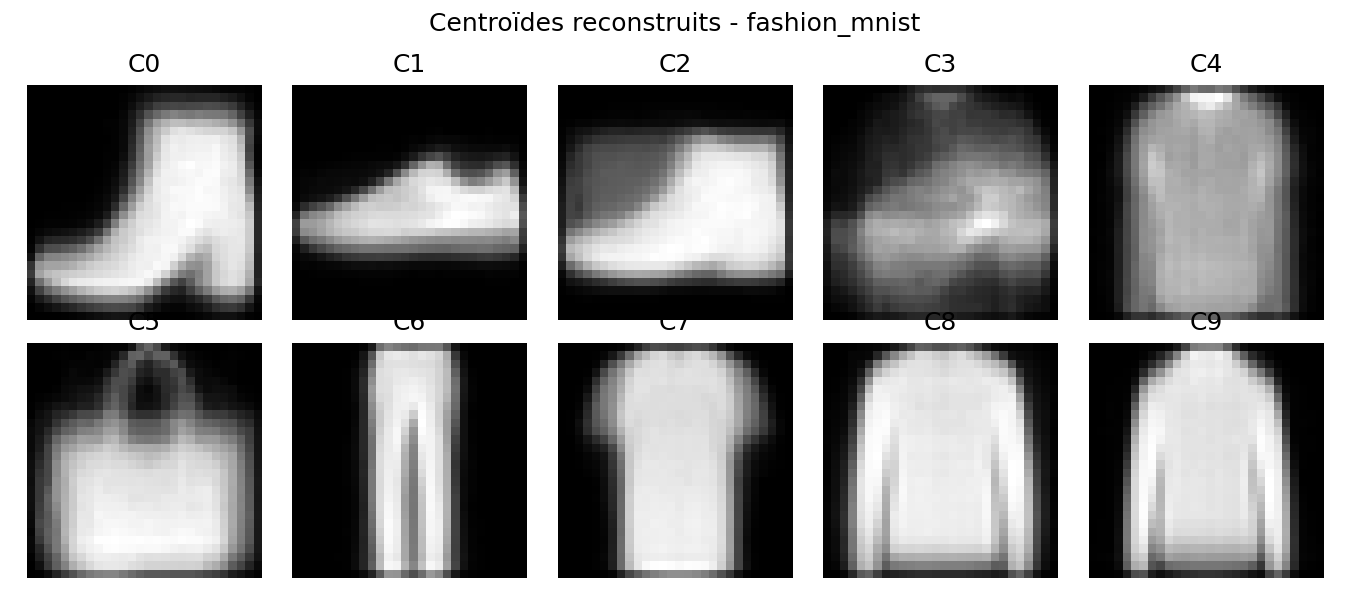
\includegraphics[width=.46\textwidth]{clustering_fashion_mnist_centroides.png}
\caption{Centroïdes obtenus sur les deux jeux d'images.}
\end{figure}

\section{Conclusion}
Ce TP m'a permis de comprendre que le choix du modèle est très important. Par
exemple, changer OLS par RBF améliore beaucoup le jeu Nonlinear. J'ai aussi vu
que le nombre d'époques ne suffit pas pour comparer les méthodes : une époque
de GD contient une seule mise à jour, alors que SGD contient plusieurs
mini-lots.

Les méthodes adaptatives donnent souvent de bons résultats rapidement, mais
elles dépendent du pas choisi. Le clustering dépend aussi de l'initialisation.
Les moyennes et écarts types sont calculés sur les graines 42, 123 et 2024 pour
les méthodes stochastiques. Pour les méthodes déterministes, une seule exécution
est suffisante avec la même initialisation. J'ai gardé séparément le nombre de
mises à jour, les appels au gradient et les appels à la perte, car une époque de
GD n'a pas le même coût qu'une époque de SGD.
La principale limite de mes résultats est le budget court utilisé pour MNIST et
Fashion-MNIST. Le code contient un mode \texttt{full} pour lancer l'expérience
avec les partitions complètes et trois graines.

\section*{Commande d'exécution}
\begin{verbatim}
python3 run_all.py --profile quick
python3 run_all.py --profile full
\end{verbatim}

\noindent Dépôt du code :
\url{https://github.com/DevOam/optimisation-numerique-numpy}

\end{document}
